% Prof. Dr. Ausberto S. Castro Vera
% UENF - CCT - LCMAT - Curso de Ci\^{e}ncia da Computa\c{c}\~{a}o
% Campos, RJ,  2020
% Disciplina: Paradigmas de Linguagens de Programa\c{c}\~{a}o
% Aluno:



\chapterimage{ScalaH} % Chapter heading image ==>  Trocar este arquivo por outro 1200x468
\chapter{Ferramentas existentes e utilizadas}

\begin{quote}

  Neste capítulo encontrará o processo de criação desse livro, as ferramentas utilizadas para processar e visualizar os códigos que foram apresentados. Portanto, nome de ferramentas, IDE, compiladores e suas versões serão apresentados a seguir.
  \hspace{2.5mm} Em cada caso será levado em consideração os seguintes critérios:
  \begin{itemize}
    \item Nome da ferramenta (compilador-interpretador);
    \item Vers\~{a}o atual e utilizada;
    \item Captura de tela da ferramenta;
    \item Informa\c{c}\~{o}es adicionais.
  \end{itemize}
\end{quote}


\section{Editores para Scala}
\begin{quote}
  No processo de desenvolvimento das aplicações e programação apresentados neste livro foi utilizado a ferramenta de edição Visual Studio Code na sua última versão “October 2021 (version 1.62)”.
  Visual Studio Code é um editor de código-fonte da Microsoft para Windows, Linux e macOS. Os recursos incluem suporte para depuração, realce de sintaxe, autocompletar de código inteligente, snippets, refatoração de código e Git incorporado.
  Link para o site oficial: \href{https://code.visualstudio.com/}{Visual Studio Code - Code Editing.}
  \begin{figure}[H]
    \begin{center}
      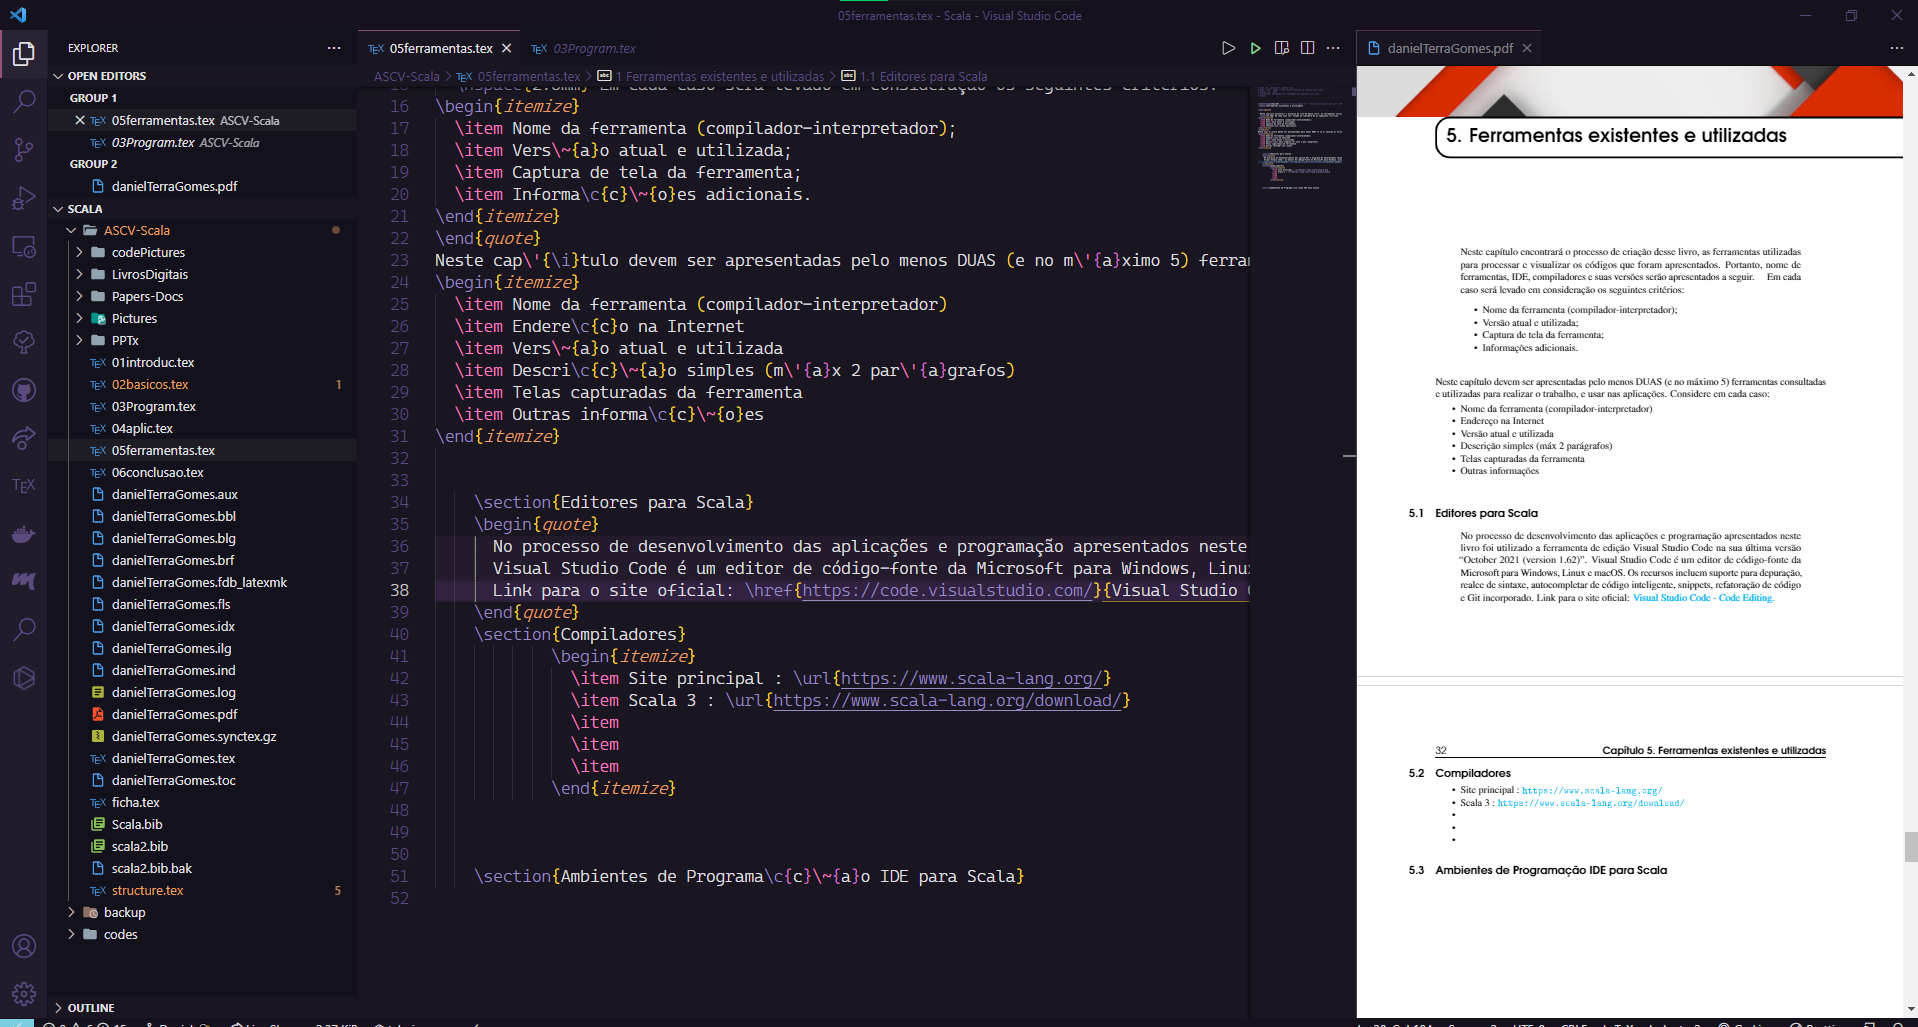
\includegraphics[width=15cm]{vscode1}
      % 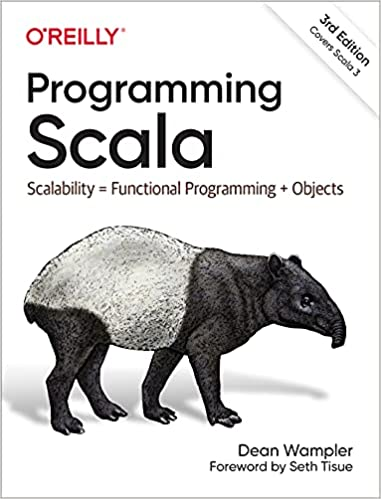
\includegraphics[width=7cm]{livro2021} \\
      \caption{Visual Studio Code - Code Editing.} \label{edit}
      {\tiny \sf Fonte: O autor }
    \end{center}
  \end{figure}
\end{quote}
\section{Compiladores}
\begin{quote}
  O códigos desenvolvidos foram compilados usando a seguinte versão do compilador Scala:
  “Scala compiler version 2.13.6 -- Copyright 2002-2021, LAMP/EPFL and Lightbend, Inc”.
  Link para o site oficial: \href{https://www.scala-lang.org/}{The Scala Programming Language}
  Ressalvo que a última versão do compilador Scala e a seguinte:  “Scala compiler version 3.1.0 -- Copyright 2002-2021, LAMP/EPFL and Lightbend, Inc.”
  \begin{figure}[H]
    \begin{center}
      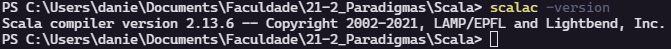
\includegraphics[width=13cm]{scalacompiler}
      \caption{Scala compiler version 2.13.6} \label{compiler}
      {\tiny \sf Fonte: O autor }
    \end{center}
  \end{figure}

\end{quote}

\section{Ambientes de Programa\c{c}\~{a}o IDE para Scala}
\begin{quote}
Uma IDE, do inglês “Integrated Development Environment”,  permite que os programadores consolidem os vários aspectos da escrita de um programa de computador. IDEs aumentam a produtividade do programador combinando atividades comuns de escrita de software em um único aplicativo: edição de código-fonte, criação de executáveis e depuração.

\hspace{2.5mm} NetBeans:

O NetBeans IDE permite que os desenvolvedores desenvolvam de forma rápida e fácil aplicativos de desktop, móveis e web. Graças às suas muitas funções de edição, análise e conversão, o NetBeans IDE torna o trabalho mais fácil para os desenvolvedores. A ferramenta de gerenciamento de projetos por si só vale a pena dar uma olhada.

O plug-in Scala para NetBeans oferece um editor Scala completo com sintaxe e coloração semântica, um navegador de estrutura de tópicos, autocompletar código e muito mais. Há também um depurador, console interativo e integração com Junit e Maven.

\hspace{2.5mm} IDE Scala para Eclipse:

Há, também, uma extensão Scala para Eclipse.
Esta IDE Scala oferece suporte dedicado para o desenvolvimento de Scala puro e aplicativos mistos. Scala IDE oferece aos desenvolvedores uma variedade de ferramentas e recursos, bem como algumas notaveis correcoes de bugs.
Ferramentas de edição avançadas incluem autocompletar código, realce implícito e semântico e um guia de indentação completamente novo. Há um depurador Scala brilhante para facilitar sua vida, junto com um localizador de teste Junit confiável e depurador assíncrono.



\end{quote}
